\documentclass{article}
\usepackage{graphicx}
\usepackage{listings}
\usepackage{color}
\usepackage[margin=1.5in]{geometry} 

\usepackage{hyperref}
\hypersetup{colorlinks,urlcolor=blue,linkcolor=}

\definecolor{listinggray}{gray}{0.9}
\definecolor{graphgray}{gray}{0.7}
\definecolor{blue}{rgb}{0,0,1}

\newcommand{\Jcode}[3]{
  \lstset{language=Java}
  \lstset{backgroundcolor=\color{listinggray},rulecolor=\color{blue}}
  \lstset{linewidth=\textwidth}
  \lstset{commentstyle=\textit, stringstyle=\upshape,showspaces=false}
  \lstset{frame=tb}
  \lstinputlisting[caption={#1},label={#2}]{#3}
}

\author{Matthew Mosley, Trey Sanchez}
\title{WBAN for Android Documentation}
\begin{document}
\maketitle

\def \WID {1.7in}
\section{Usage}
The WBAN application performs the following functions:

\begin{itemize}
\item plot data in real time
\item display historical data
\item allow user to email data
\item stores data in a comma separated file
\end{itemize}

When the user starts up the app, he will see the start screen shown in Figure \ref{fig:start}.

\begin{figure}[!h]
\label{fig:start}
  \centering
  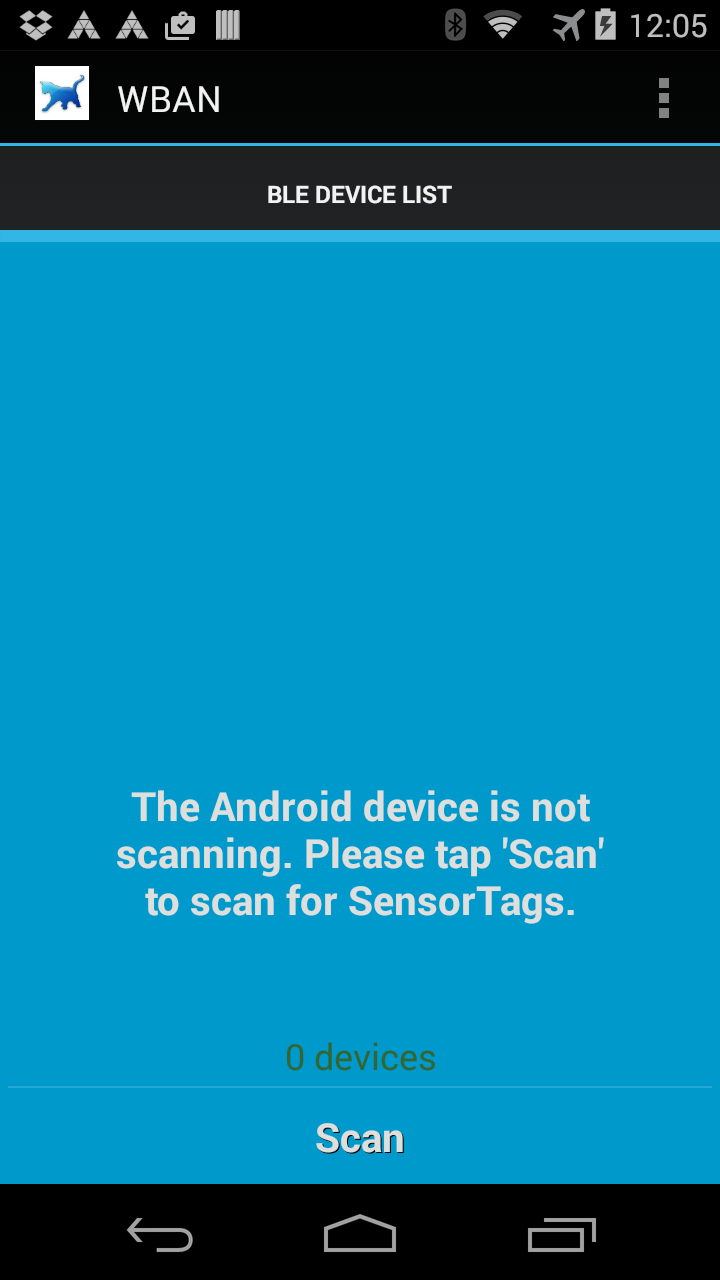
\includegraphics[width=\WID]{pics/start.png}
  \caption{Start screen}
\end{figure}

The user should press the scan button and the app will use the phone's bluetooth adapter to scan for devices. When
it finds the sensor tag, the sensor tag will display as in Figure \ref{fig:scan}.

\begin{figure}[!h]
  \centering
  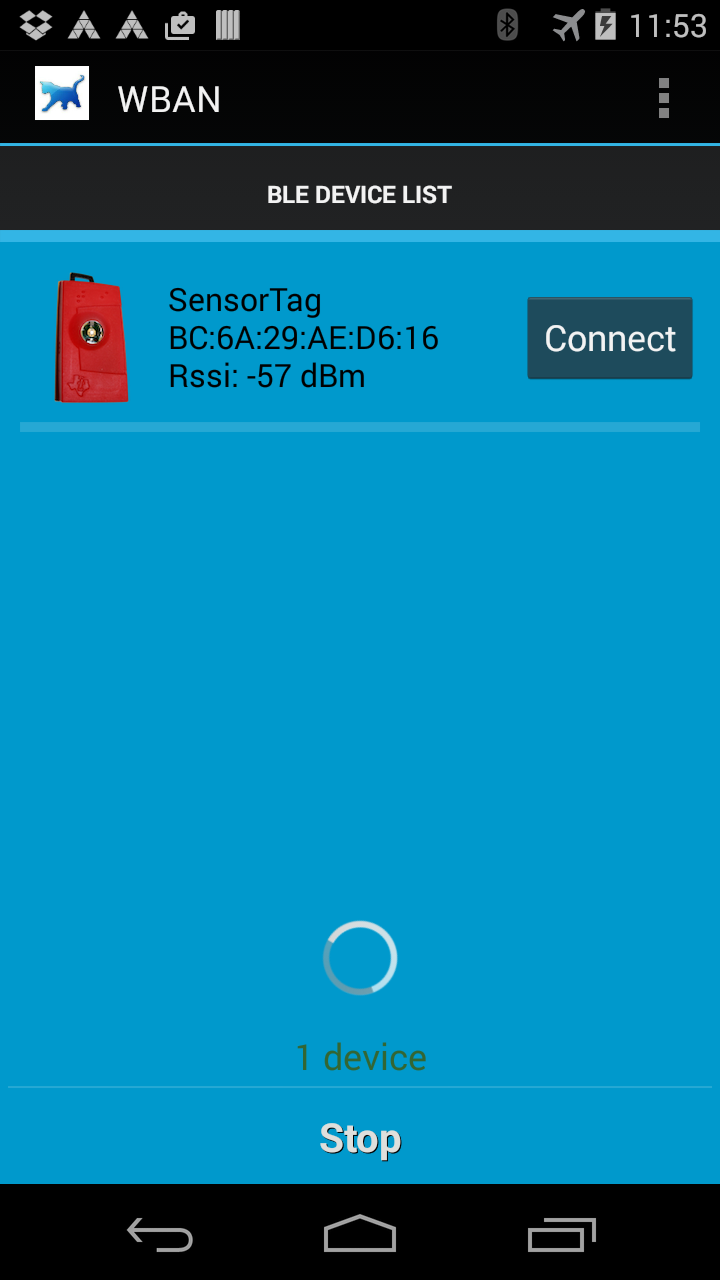
\includegraphics[width=\WID]{pics/scan.png}
  \caption{Device detected}
  \label{fig:scan}
\end{figure}

The user then presses ``Connect'' and is then taken to the selection screen.

\begin{figure}[!h]
  \centering
  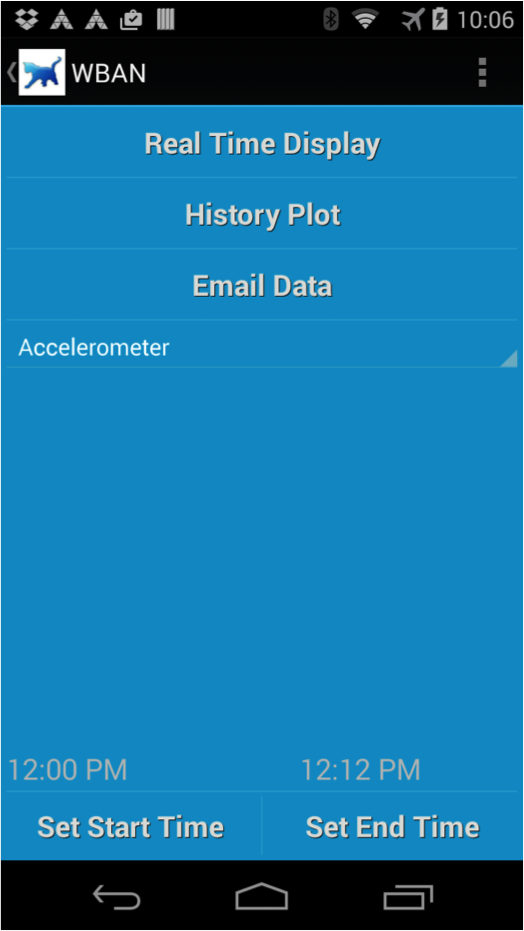
\includegraphics[width=\WID]{pics/select.png}
  \caption{Selection screen}
  \label{fig:select}
\end{figure}

From the selection screen, the user can choose from the following options:

\begin{itemize}
\item Real Time Display - display data in real time for the currently selected sensor
\item History Plot - display historical data 
\item Email Data - email the data in a zip file to a designated recipient
\item Sensor Selector - choose which sensor to plot data from
\end{itemize}

While in the selection screen, the app is continuously listening for incoming data and saving it to a
comma-separated file named wbandata.csv. The location of this file is in the Downloads folder. It can be changed by
modifying the ``PATH'' constant in DeviceActivity.java:


\section{Developer Notes}
The WBAN application allows additional sensors to be added (e.g., heart rate, temperature). They should be added in
the code within the following methods in DeviceActivity.java

\Jcode{onItemSelected}{OIS}{code/OIS.java}

\Jcode{updatePlot}{UP}{code/UP.java}


The following libraries were used for the WBAN app:
\begin{itemize}
\item Android plot
\item OpenCVS
\end{itemize}

\end{document}